\documentclass{article}
\usepackage{amsmath,amssymb}
\usepackage[numbers]{natbib}
\usepackage{geometry}
 \geometry{
 a4paper,
 total={170mm,257mm},
 left=30mm,
 top=30mm,
 right=30mm,
 bottom=30mm
 }
 
\usepackage{graphicx}
\usepackage{caption}
\usepackage{subcaption}
\usepackage{float}

\setlength{\parskip}{1em}

\title{Reinforcement Learning Assignment-2 \\
	\Large Multi-Armed Bandit Problem \\}
\begin{document}
\author{Utkarsh Prakash \\ \normalsize 180030042}
\maketitle
\section{Experiment Setting}
\section{Bernoulli Reward Distribution}
	\subsection{K=2 arm Problem}
		\subsubsection{Greedy Algorithm}
		
		In this section, we compare the pure Greedy algorithm, $\epsilon$-greedy with fixed $\epsilon=0.1$ and $\epsilon=0.01$ and variable $\epsilon$ with the 
		following schedule:
		\begin{equation}
		\nonumber
			\epsilon_{t} = min\{1, \frac{C}{t}\}
		\end{equation}
		where $C=10$ and $t$ is the total number of plays. We observe the following graphs:
		
		\begin{figure}[H]
		\graphicspath{ {../Experiments/Bernoulli_2_Greedy/} }
		\centering
		\begin{minipage}{.5\textwidth}
		  \centering
		  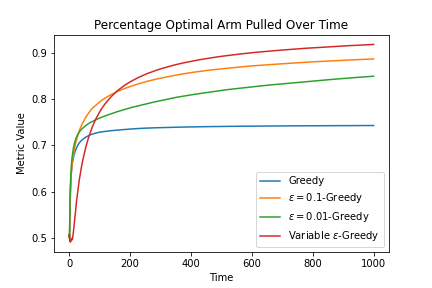
\includegraphics[width=\linewidth]{Percentage_Optimal_Arm_Pulled_Over_Time.png}
		  \captionof{figure}{Percentage Optimal Arm Pulled Over Time}
		  \label{fig:test1}
		\end{minipage}%
		\begin{minipage}{.5\textwidth}
		  \centering
		  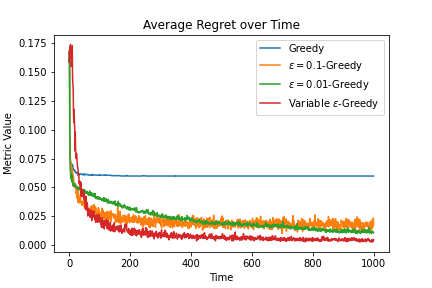
\includegraphics[width=\linewidth]{Average_Regret_over_Time.png}
		  \captionof{figure}{Average Regret over Time}
		  \label{fig:test2}
		\end{minipage}
		\end{figure}
		
		\textbf{Observations:}
		\begin{itemize}
			\item The variable $\epsilon$-Greedy tends to perform better than all of its counter-parts.
			\item In general, $\epsilon$-Greedy performs better than pure Greedy because of its tendency to explore the arms along with exploting the current 
				known knowledge.
		\end{itemize}
		
		
		\subsubsection{Softmax Policy}
		
		In this section, we compare the Softmax Policy which is defined as follows:
		\begin{equation}
		\nonumber
			\pi_{t}(a) = \frac{e^{q_{t}(a)/\tau}}{\sum_{i=1}^{K} e^{q_{t}(a_{i})/\tau}}
		\end{equation}
		where $\tau$ is the temperature hyperparameter. We compare the performance of Softmax Policy for $\tau=0.01$, $\tau=10000$ and variable $\tau$ with following
		schedule:
		\begin{equation}
		\nonumber
			\tau_{t} = \frac{C}{t}
		\end{equation}
		where $C=10$. We reduce the $\tau$ overtime to control exploration-exploitation tradeoff. The graph for different metrics are obtained as follows:
		
		\begin{figure}[H]
		\graphicspath{ {../Experiments/Bernoulli_2_Softmax/} }
		\centering
		\begin{minipage}{.5\textwidth}
		  \centering
		  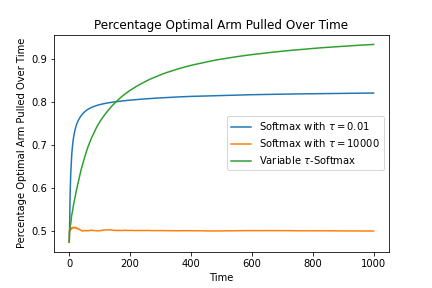
\includegraphics[width=\linewidth]{Percentage_Optimal_Arm_Pulled_Over_Time.png}
		  \captionof{figure}{Percentage Optimal Arm Pulled Over Time}
		  \label{fig:test1}
		\end{minipage}%
		\begin{minipage}{.5\textwidth}
		  \centering
		  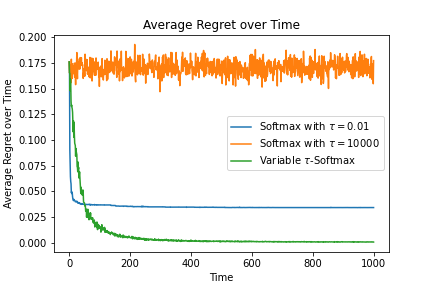
\includegraphics[width=\linewidth]{Average_Regret_over_Time.png}
		  \captionof{figure}{Average Regret over Time}
		  \label{fig:test2}
		\end{minipage}
		\end{figure}
		
		\textbf{Observations:}
		\begin{itemize}
			\item For small values of $\tau=0.01$, the algorithm performs poorly because in the limit when $\tau \to 0$, then the algorithm performs greedily.
			\item For large values of $\tau=10,000$, the algorithm performs poorly because in the limit when $\tau \to \infty$, then the algorithm picks an arm
				uniformly at random. Therefore, for such large values of $\tau$ the algorithm explores at lot.
			\item The variable $\tau$-Softmax tends to perform better than all of its counter-parts. This is because earlier when the value of $\tau$ is high, we
			tend to explore more, whereas as time progresses and we gather knowledge of different arms, we reduce the value of $\tau$ so as to exploit the knowledge
			that we have gathered (i.e., pull the arm which has highest estimated average reward with high probability).
		\end{itemize}
		
		
		\subsubsection{UCB Algorithm}
		In this section we compare the UCB algorithm where we pick the arm which has the highest value of 
		\begin{equation}
		\nonumber
			\arg max_{a \in \mathcal{A}} \left (q_{t}(a) + C\sqrt{\frac{2 \ln t}{n_{t}(a)}} \right )
		\end{equation}
		where $C$ is a hyperparameter which controls exploration-exploitation tradeoff. We used three different values of $C$ (1, 100 and variable). The graphs 
		obtained are as follows:
		
		\begin{figure}[H]
		\graphicspath{ {../Experiments/Bernoulli_2_UCB/} }
		\centering
		\begin{minipage}{.5\textwidth}
		  \centering
		  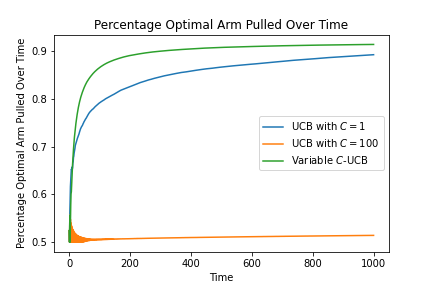
\includegraphics[width=\linewidth]{Percentage_Optimal_Arm_Pulled_Over_Time.png}
		  \captionof{figure}{Percentage Optimal Arm Pulled Over Time}
		  \label{fig:test1}
		\end{minipage}%
		\begin{minipage}{.5\textwidth}
		  \centering
		  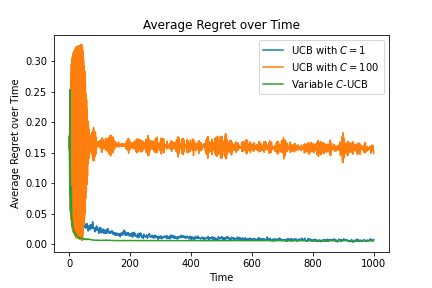
\includegraphics[width=\linewidth]{Average_Regret_over_Time.png}
		  \captionof{figure}{Average Regret over Time}
		  \label{fig:test2}
		\end{minipage}
		\end{figure}
		
		\textbf{Observations:}
		\begin{itemize}
			\item We can see the variable-$C$-UCB algorithm outperforms its counter-parts.
			\item For large values of $C=100$, the algorithm performs poorly because it explores too much.
		\end{itemize}
		
		\subsubsection{Thompson Sampling}
		In Thompson Sampling, we maintain a Beta distribution prior over $q_{t}(a)$. We sample a value $Q_{t}(a)$ from this Beta distribution for each arm, i.e.
		$q_{t}(a) \stackrel{}{\sim} Q_{t}(a)$. Now, we select the arm which has the highest value of $Q_{t}(a)$. The results obtained for this algorithm is as 
		follows:
		
		\begin{figure}[H]
		\graphicspath{ {../Experiments/Bernoulli_2_Thompson_Sampling/} }
		\centering
		\begin{minipage}{.5\textwidth}
		  \centering
		  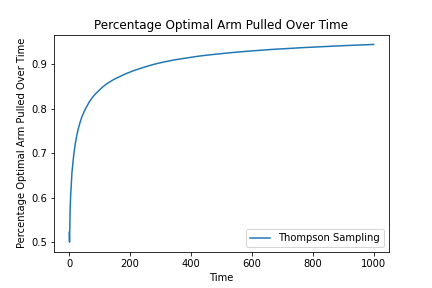
\includegraphics[width=\linewidth]{Percentage_Optimal_Arm_Pulled_Over_Time.png}
		  \captionof{figure}{Percentage Optimal Arm Pulled Over Time}
		  \label{fig:test1}
		\end{minipage}%
		\begin{minipage}{.5\textwidth}
		  \centering
		  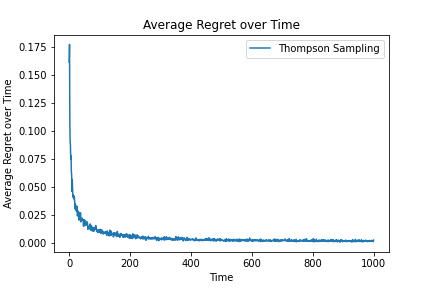
\includegraphics[width=\linewidth]{Average_Regret_over_Time.png}
		  \captionof{figure}{Average Regret over Time}
		  \label{fig:test2}
		\end{minipage}
		\end{figure}
		
		\subsubsection{Reinforce Algorithm}
		
		\begin{equation}
		\nonumber
		\end{equation}
		
		\begin{itemize}
			\item
		\end{itemize}
\end{document}